%!TEX root = ../notes.tex
\section{January 31, 2023}
\label{20230131}
\subsection{Logistics}
There's an EdStem post asking about topics you're interested, feel free to keep on posting!

We acknowledge the synchronization issues with Panopto. For now, if you want to watch the lecture recordings, you can use the Zoom link linked from the course home page. We can manually sync up EdStem but Panopto cannot be synced up, unfortunately.

\subsection{Encryption Schemes}
This lecture we'll cover encryption schemes. We briefly mentioned what encryption schemes were last class, we'll dive into the technical content: how we construct them, assumptions, RSA, ElGamal, etc.

Fundamentally, an encryption scheme protects message secrecy. If Alice wants to communicate to Bob, Alice will encrypt a message (plaintext) using some key which gives her a ciphertext. Sending the ciphertext through Bob using a public channel, Bob can use the key to decrypt the ciphertext and recover the message. An eavesdropper in the middle will have no idea what message has been transmitted.

\begin{center}
    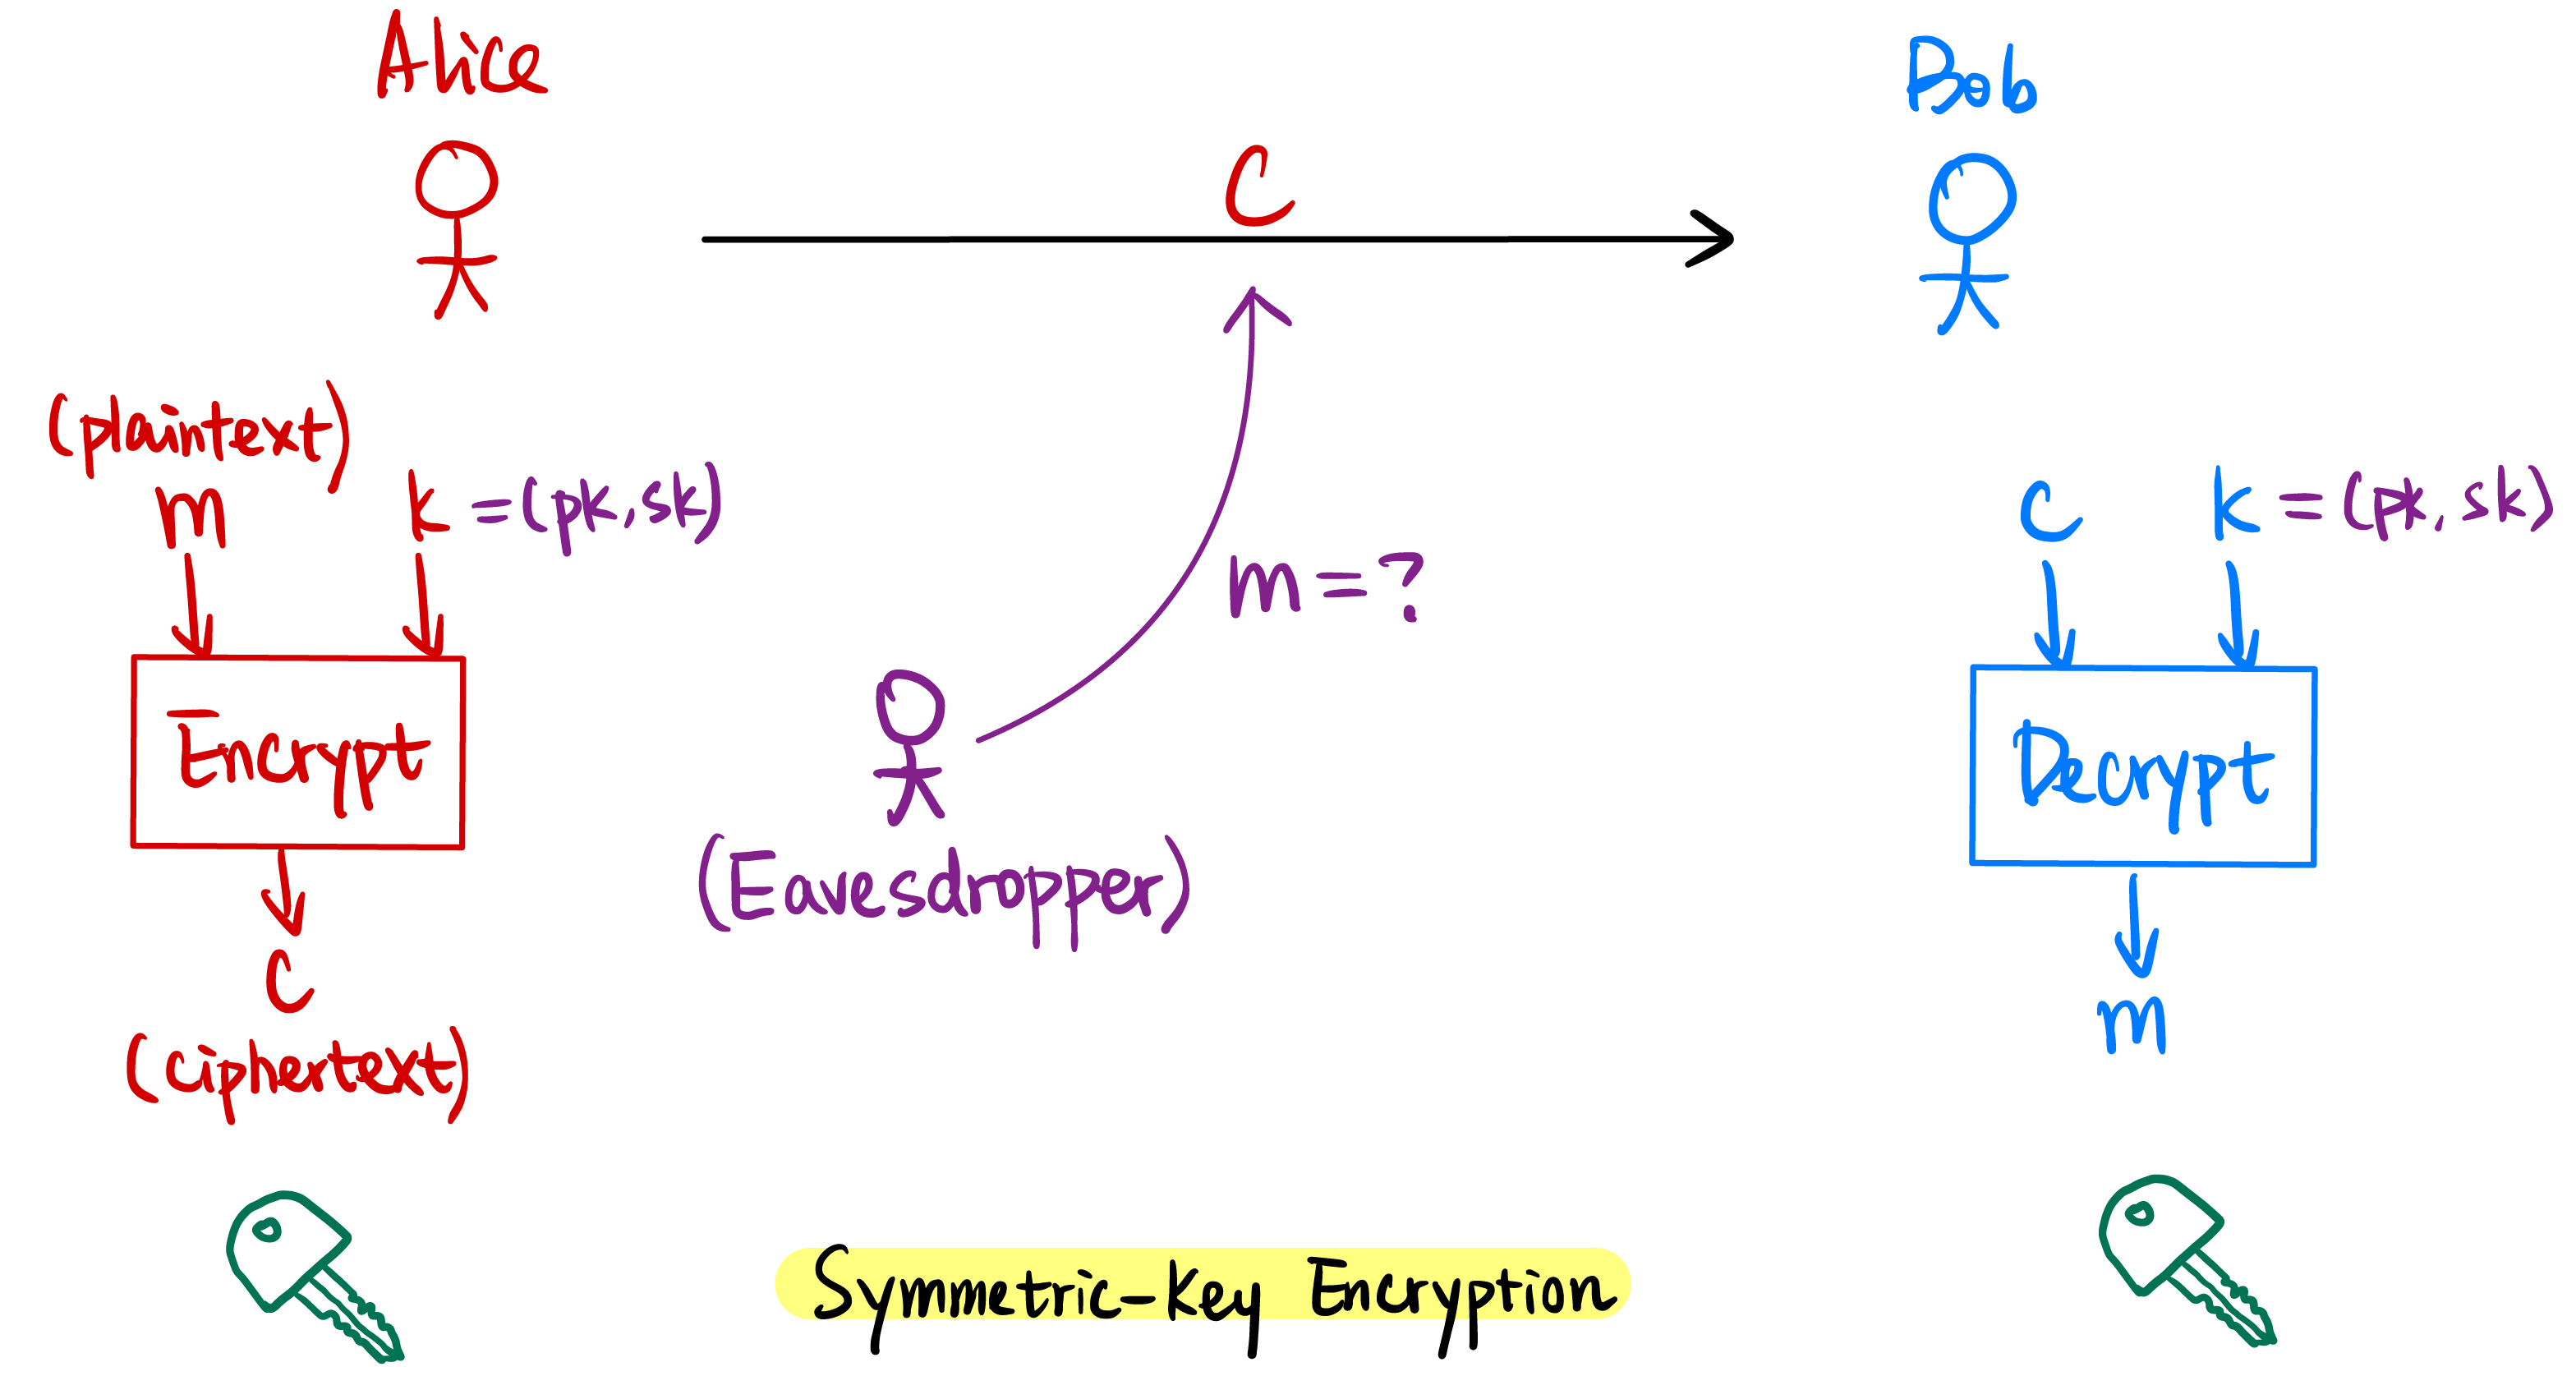
\includegraphics[width=0.8\textwidth]{images/2023-01-31/ske-intro.png}
\end{center}

In this case, they are using a shared key, which we called secret-key encryption or symmetric-key encryption.

A stronger version of private-key encryption is called public-key encryption. Alice and Bob do not need to agree on a shared secret key beforehand. There is a keypair $(pk, sk)$, a \emph{public} and \emph{private} key.

\begin{center}
    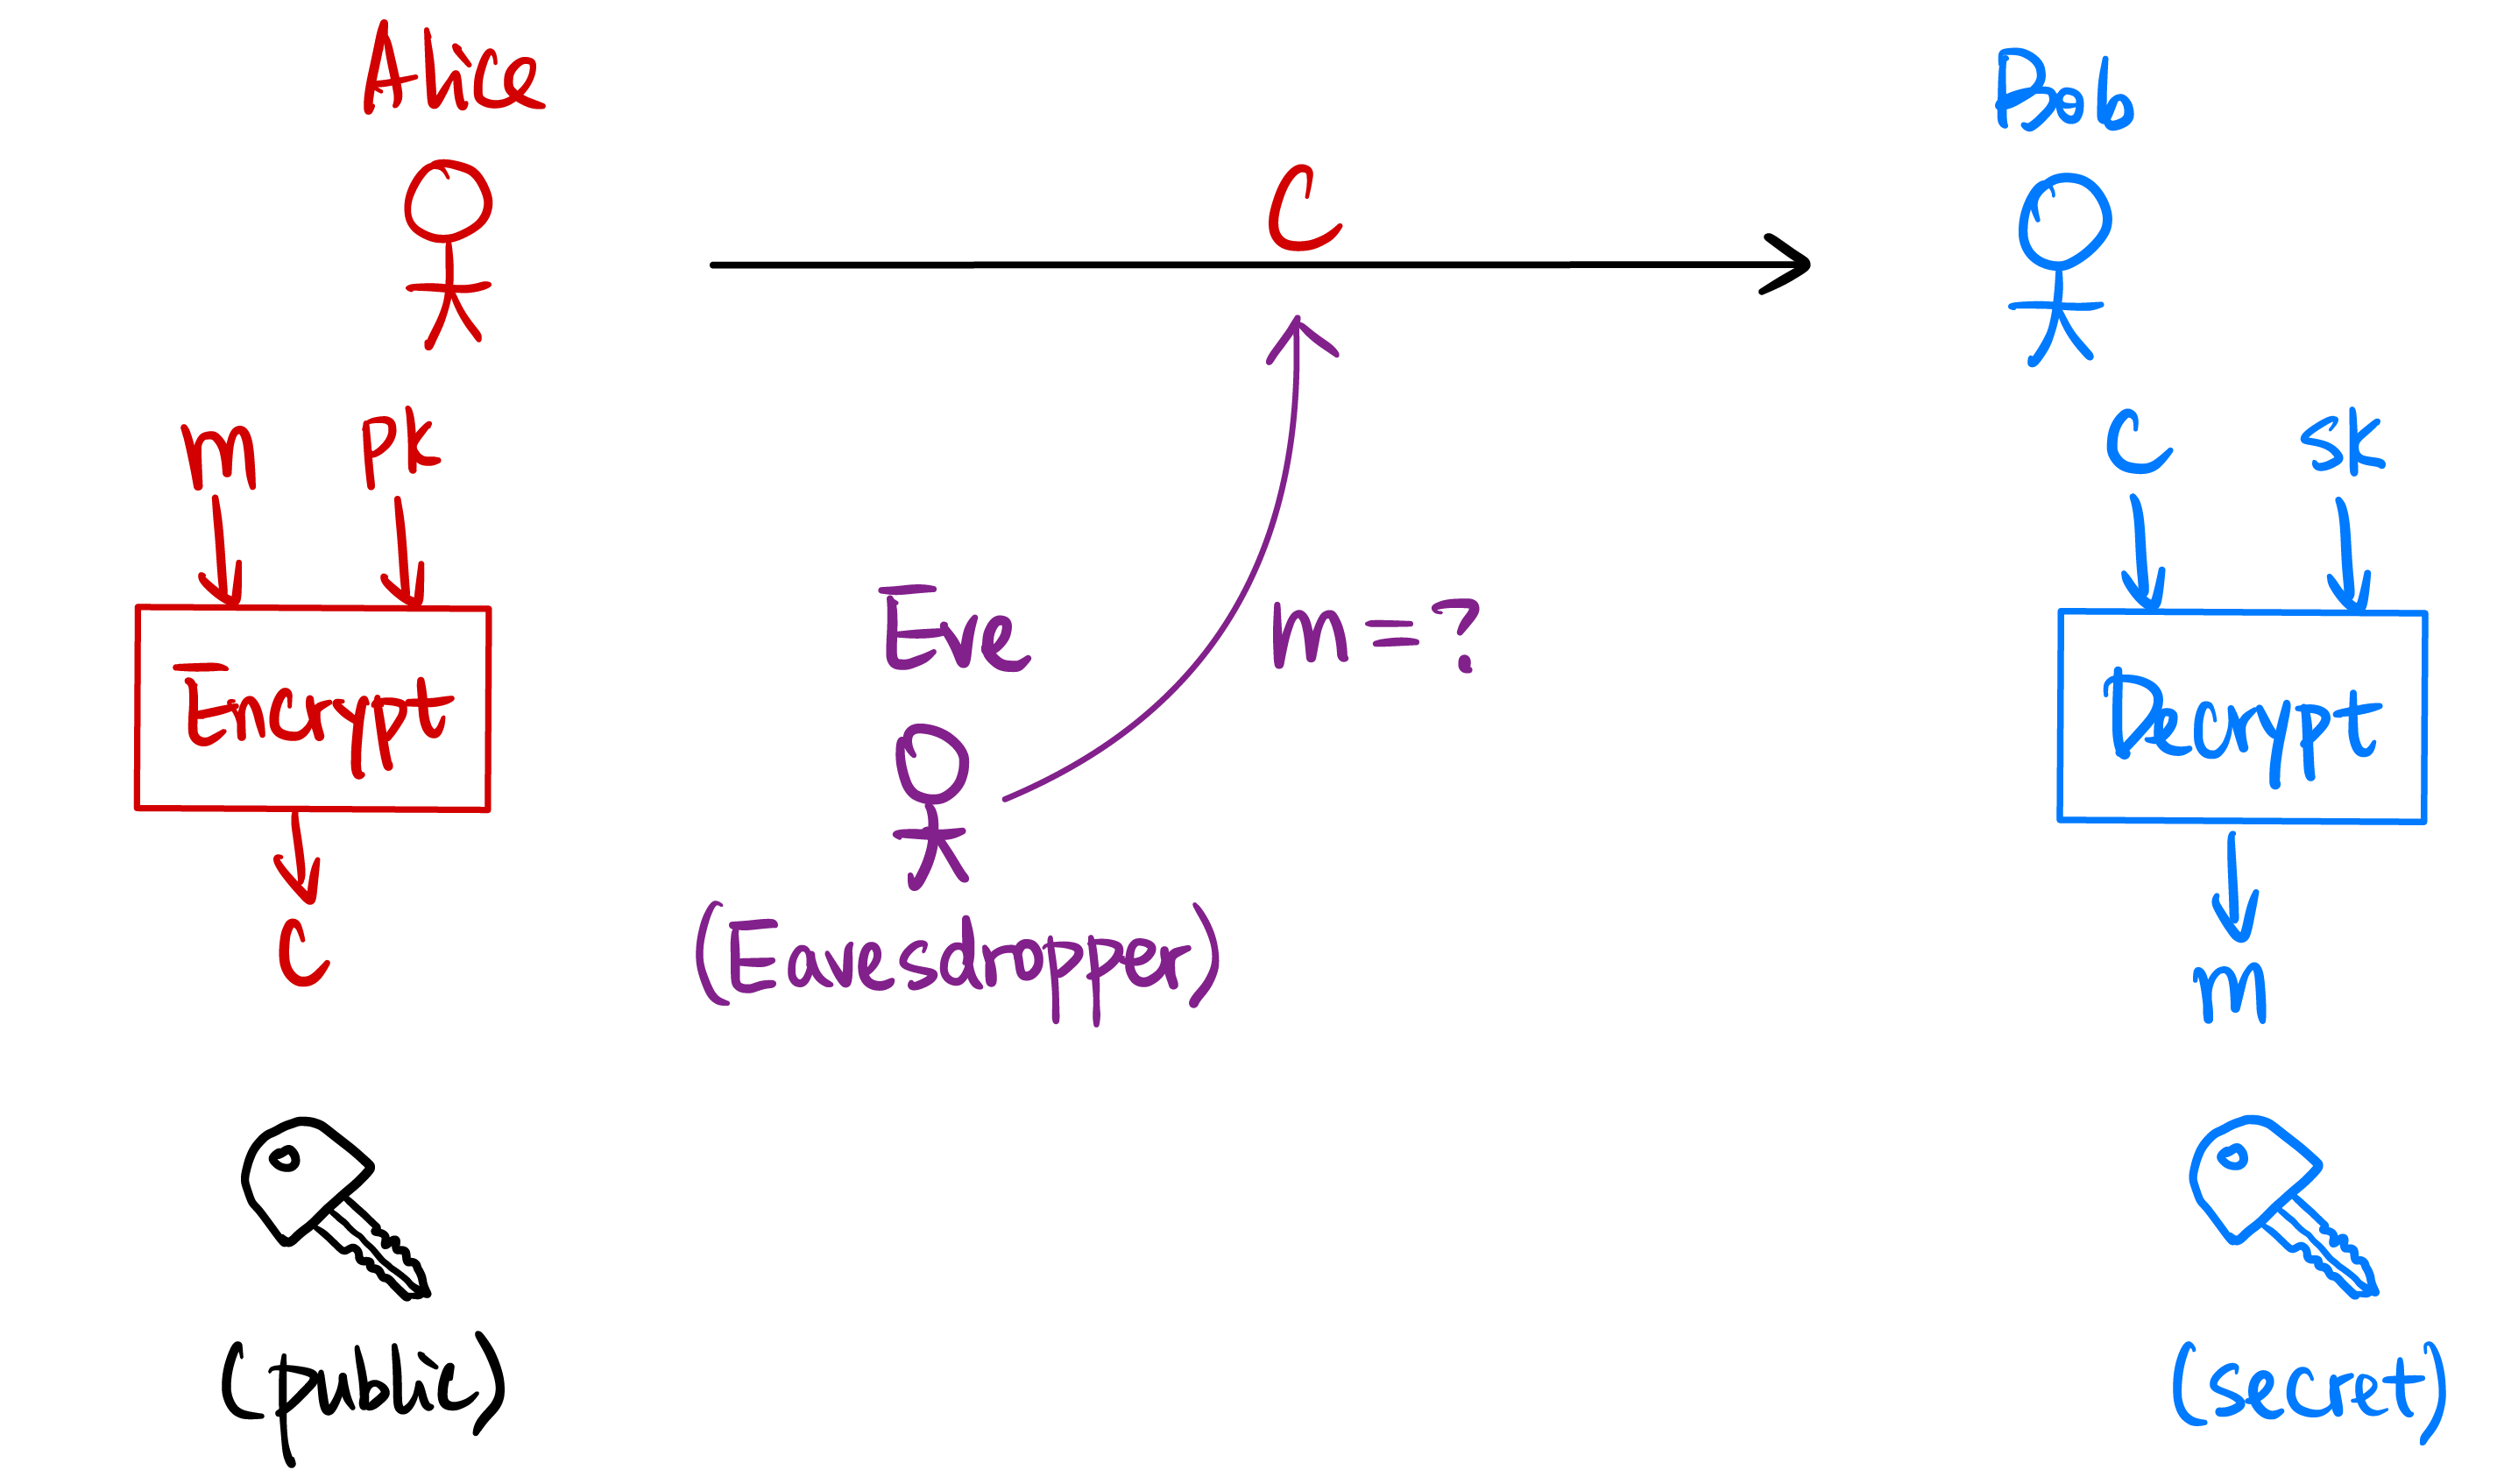
\includegraphics[width=0.8\textwidth]{images/2023-01-31/pke-intro.png}
\end{center}

\subsubsection{Syntax}
\begin{definition}[Symmetric-Key Encryption]
    A symmetric-key encryption (SKE) scheme contains 3 algorithms, $\pi = (\mathsf{Gen}, \mathsf{Enc}, \mathsf{Dec})$.

    \begin{description}
        \item[Generation.] Generates key $k\leftarrow \mathsf{Gen}$.
        \item[Encryption.] Encrypts message $m$ with key $k$, $c\leftarrow \mathsf{Enc}(k, m)$, which we sometimes write as $\Enc_k(m)$.
        \item[Decryption.] Decrypts using key $k$ to retrieve message $m$, $m := \Dec(k, c)$, or written as $\Dec_k(c)$.
    \end{description}
    Note the notation $\leftarrow$ and $:=$ is different. In the case of generation and encryption, the produced key $k$ or $c$ follows a \emph{distribution} (is randomly sampled), but we had better want decryption to be deterministic in producing the message.
\end{definition}

\begin{definition}[Public-Key Encryption]
    A public-key encryption (PKE) scheme $\pi = (\Gen, \Enc, \Dec)$ contains the same $3$ algorithms,

    \begin{description}
        \item[Generation.] Generate keys $(pk, sk)\leftarrow \Gen$.
        \item[Encryption.] Use the public key to encrypt, $c\leftarrow \mathsf{Enc}(pk, m)$ or $\Enc_{pk}(m)$.
        \item[Decryption.] Use the secret key to decrypt, $m:=\Dec(pk, c)$ or $\Dec_{pk}(c)$.
    \end{description}

\end{definition}

\begin{ques*}
    If we can construct public-key encryption, why do we even bother with secret-key encryption? We could just use the $(pk, sk)$ pair for our secret key, and this does the same thing.
\end{ques*}

\begin{enumerate}
    \item First of all, public-key encryption is almost always \emph{more expensive}. Symmetric-key encryption schemes give us efficiency.
    \item Public-key encryption relies on much stronger computational assumptions.
\end{enumerate}

\subsubsection{Symmetric-Key Encryption Schemes}
\begin{definition}[One-Time Pad]
    Secret key is a uniformly randomly sampled $n$ bit string $k\sampledfrom \{0, 1\}^n$.

    \begin{center}
        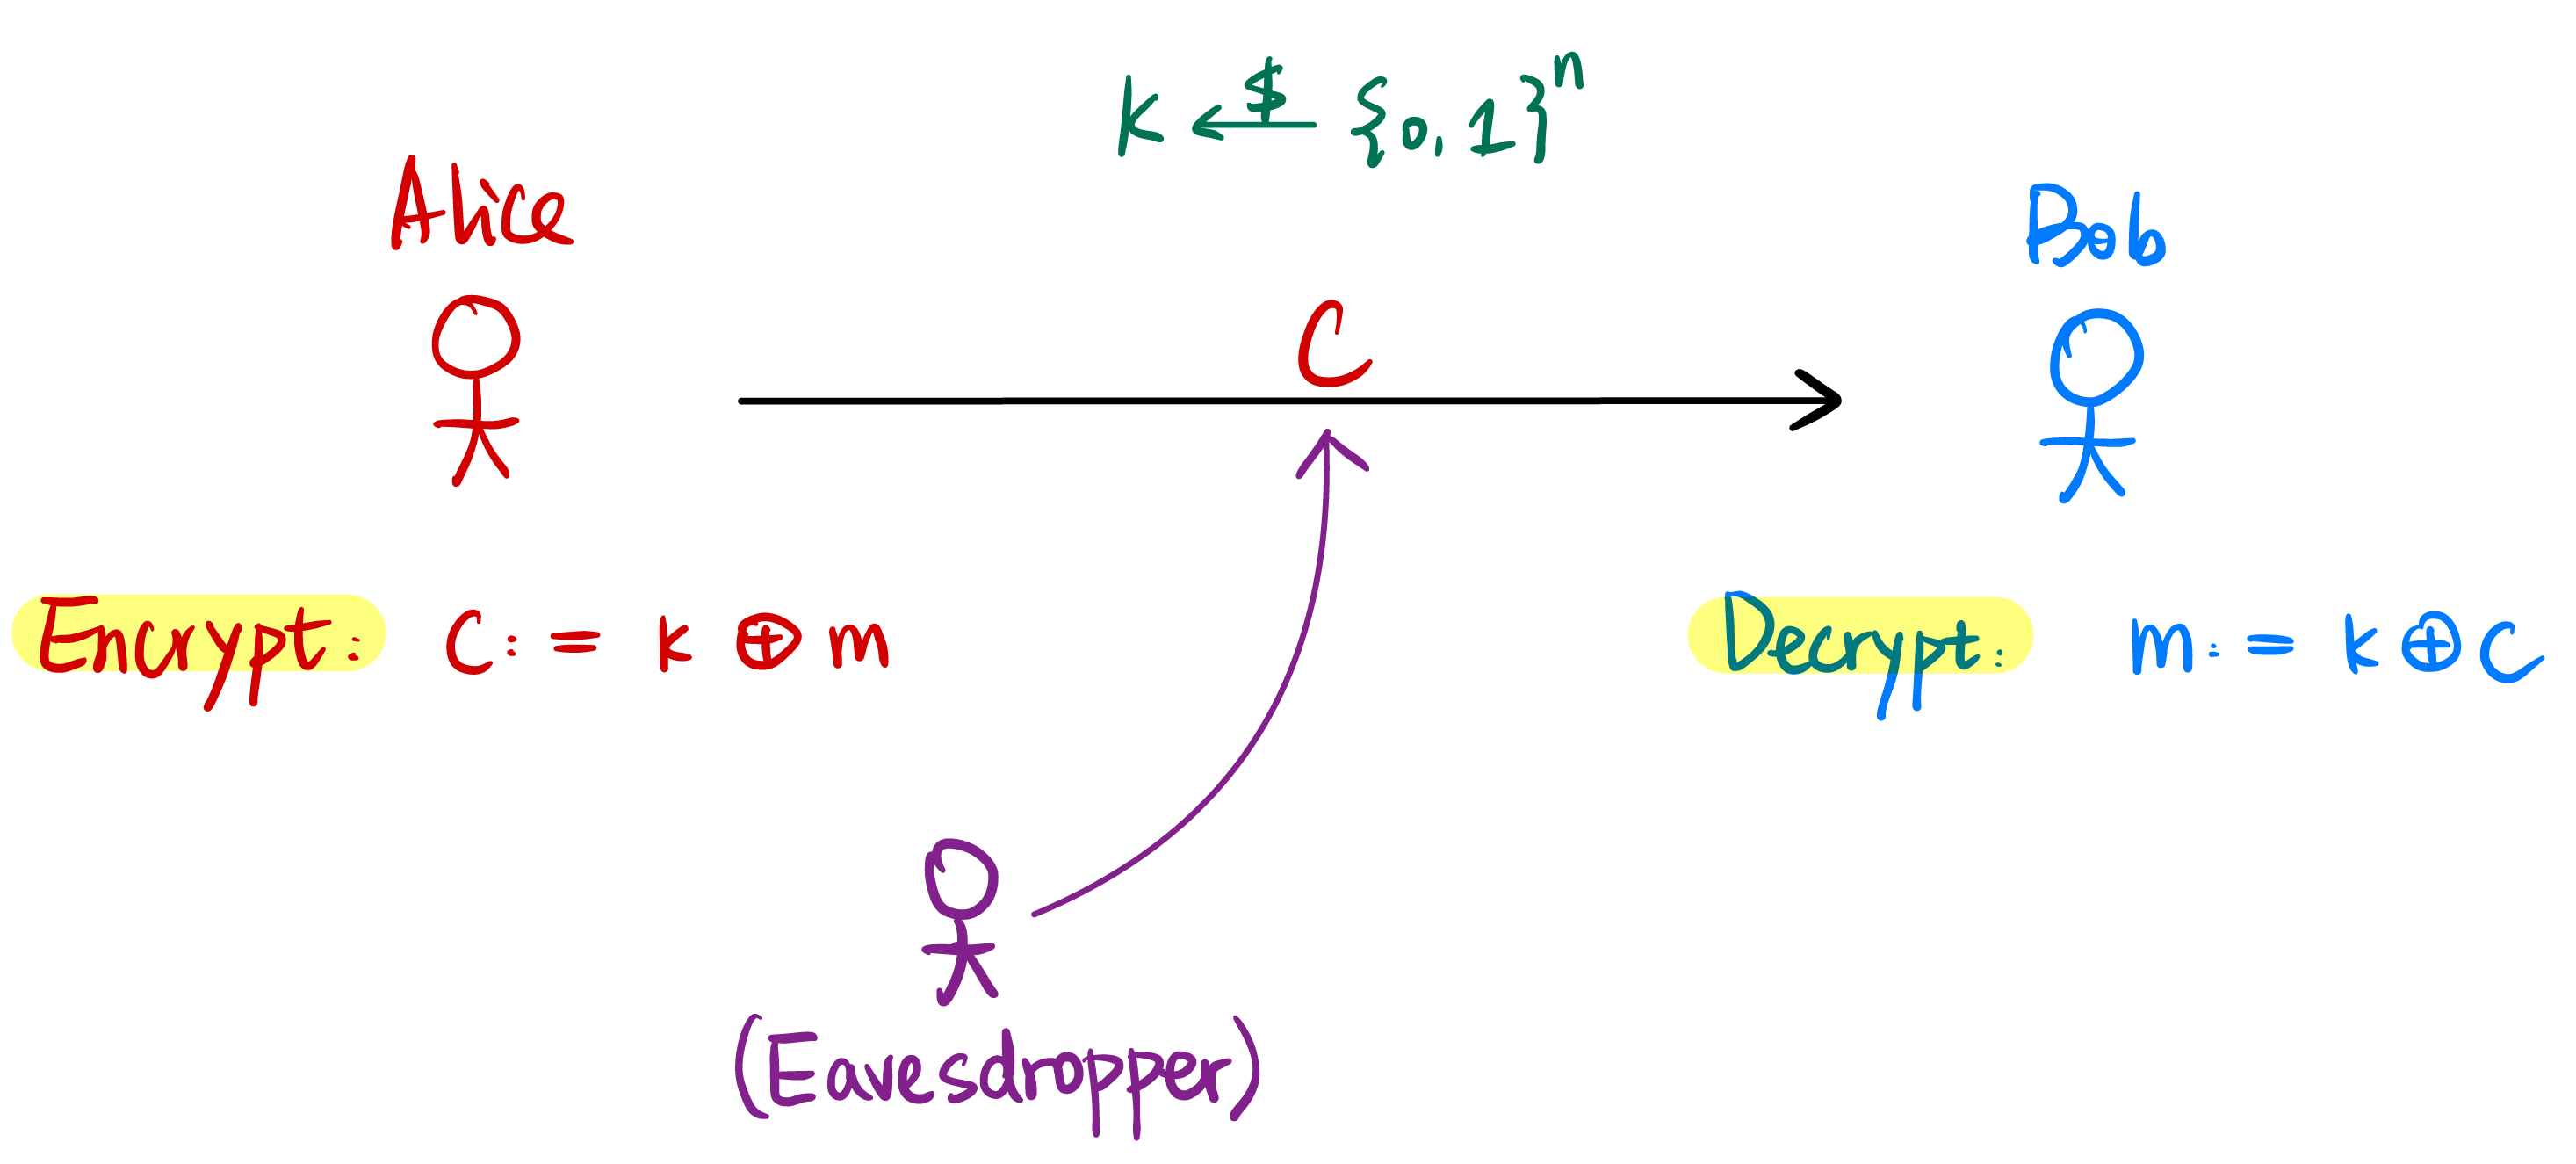
\includegraphics[width=0.7\textwidth]{images/2023-01-31/otp-defn.png}
    \end{center}

    \begin{description}
        \item[Encryption.] Alice uses the secret key and bitwise-$\mathsf{XOR}$ with the plaintext.
            \begin{align*}
                \begin{split}
                    \text{secret key}\quad k       & = 0100101 \\
                    \oplus\text{ plaintext}\quad m & = 1001001 \\ \eqline
                    \text{ciphertext}\quad c       & = 1101100
                \end{split}
            \end{align*}
        \item[Decryption.] Bob uses the secret key and again bitwise-$\mathsf{XOR}$ with the ciphertext
            \begin{align*}
                \begin{split}
                    \text{secret key}\quad k        & = 0100101 \\
                    \oplus\text{ ciphertext}\quad c & = 1101100 \\ \eqline
                    \text{plaintext}\quad c         & = 1001001
                \end{split}
            \end{align*}
    \end{description}

    This is widely used in cryptography, called \emph{masking} or \emph{unmasking}.
\end{definition}

\begin{ques*}
    Why is this correct?
\end{ques*}
An $\mathsf{XOR}$ done twice with the same choice bit $b$ is the identity. Or, an element is its own inverse with the $\mathsf{XOR}$ operator.

\begin{ques*}
    Why is this secure?
\end{ques*}

We can think about this as the distribution of $c$. $\forall m\in \{0, 1\}^n$, the encryption of $m$ is uniform over $\{0, 1\}^n$ (since $k$ was uniform).

Another way to think about this is that for any two messages $m_0, m_1\in\{0, 1\}^n$, $\Enc_k(m_0)\equiv \Enc_k(m_1)$. That is, the encryptions follow the \emph{exact same} distribution. In this case, they are both uniform, but this is not always the case.

\begin{ques*}
    Can we reuse $k$? Should we use the same key again to encrypt another message? Or, it is possible for the eavesdropper to extract information.
\end{ques*}

For example, $\Enc_k(m)$ is $c:= k\oplus m$, and $\Enc_k(m')$ is $c' := k\oplus m'$. If the two messages are the same, the ciphertexts are the same.

By $\mathsf{XOR}$ $c$ and $c'$, we get
\begin{align*}
    c\oplus c' & = (\cancel{k}\oplus m) \oplus (\cancel{k}\oplus m') \\
               & = m\oplus m'
\end{align*}
This is why this is an \emph{one-time} pad. This is a bit of an issue, to send an $n$-bit message, we need to agree on an $n$-bit message.

In fact, this is \emph{the best} that we can do.

\begin{theorem}
    \emph{Informally,} for perfect (information-theoretic\footnote{That the distributions of ciphertexts are identical, that $\Enc_k(m_0)\equiv \Enc_k(m_1)$.}) security, the key space must be at least as large as the message space.
    \[|\mathcal{K}|\geq |\mathcal{M}|\]
    where $\mathcal{K}$ is the key space and $\mathcal{M}$ is the message space.
\end{theorem}

\begin{ques*}
    How can we circumvent this issue?
\end{ques*}

The high level idea is that we weaken our security guarantees \emph{a little}. Instead of saying that they have to be \emph{exactly the same} distribution, we say that they are \emph{hard to distinguish} for an adversary with limited computational power. This is how modern cryptography gets around these lower bounds in classical cryptography. We can make \emph{computational assumptions} about cryptography.

We can think about computational security,
\begin{definition}[Computational Security]\label{def:computational-security}
    We have \ul{computational security} when two ciphertexts have distribution that cannot be distinguished using a polynomial-time algorithm.
\end{definition}

\begin{definition}[Polynomial-Time Algorithm]
    A polynomial time algorithm $A(x)$ is one that takes input $x$ of length $n$, $A$'s running time is $O(n^c)$ for a constant $c$.
\end{definition}
\begin{definition}[\textsf{NP} Problem]
    A decision problem is in \ul{nondeterministic polynomial-time} when its solution can be \emph{verified} in polynomial time.
\end{definition}
\begin{example}[Graph 3-Coloring]
    Given a graph, does it have a $3$-coloring such that no two edges join the same color? For example,

    \begin{center}
        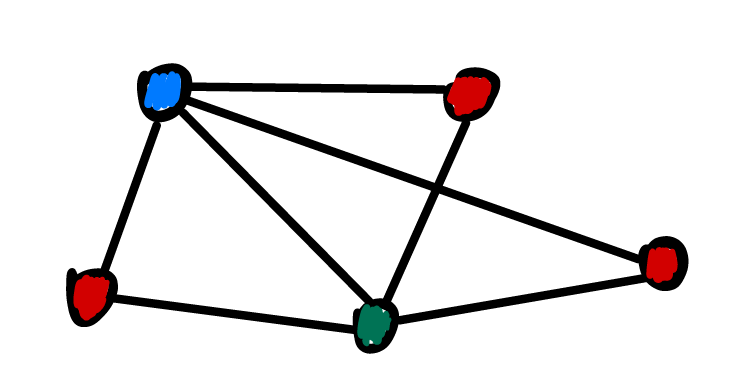
\includegraphics[width=0.4\textwidth]{images/2023-01-31/graph-coloring.png}
    \end{center}

    This can be \emph{verified} in polynomial time (we can check if such a coloring is a valid $3$-coloring), but it is computed in \textsf{NP} time.
\end{example}
\begin{definition}
    An \textsf{NP}-complete problem is a ``hardest'' problem in \textsf{NP}. Every problem in \textsf{NP} is at least as hard as an \textsf{NP}-complete problem.
\end{definition}

Right now, we assume $\mathsf{P}\neq\mathsf{NP}$. As of right now, there is no realistic algorithm that can solve any \textsf{NP} problem in polynomial-time.

Even further, we pick some problems not in $\mathsf{NP}$-complete, not in $\mathsf{P}$. We assume they are neither $\mathsf{NP}$-complete nor in $\mathsf{P}$ (we don't yet have a reduction, but we don't know if one could exist) The reasoning behind using these problems is as we have no good cryptoscheme relying solely on $\mathsf{NP}$-complete problems (we need something weaker).

\begin{center}
    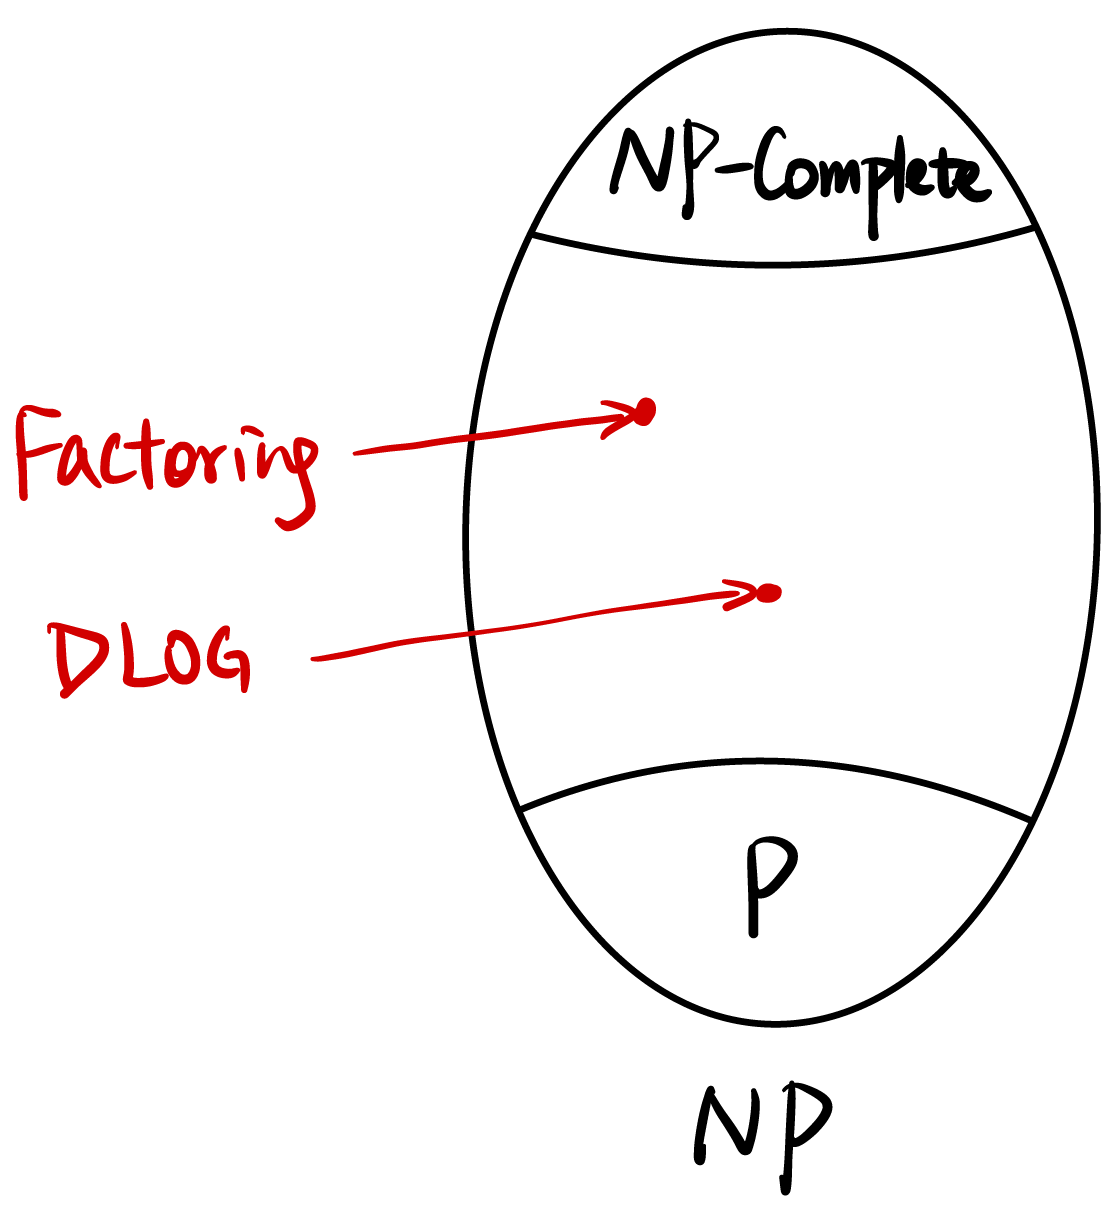
\includegraphics[width=0.4\textwidth]{images/2023-01-31/pnp-venn.png}
\end{center}

Going back to our definition of computational security \cref{def:computational-security},
\begin{definition*}[Computational Security]
    We say that the adversary is computationally bounded (is only a \emph{ polynomial-time algorithm}), that $\forall \text{probabilic poly-time algorithm }\mathcal{A}$,
    \[\Enc_k(m_0)\overset{c}{\simeq}\Enc_k(m_1)\]
    Where $\overset{c}{\simeq}$ is ``computationally indistinguishable''.
\end{definition*}

What does it mean for distributions to be ``computationally indistinguishable''? Let's say Alice encrypts multiple messages $m_0, m_1, \dots$ to Bob and produces $c_0, c_1, \dots$. Even if Eve can see all plaintexts $m_i$ in the open and ciphertexts $c_i$ in the open, between known $m_0, m_1$ and randomly encrypting one of them $c\leftarrow \Enc_{k}(m_b)$ where $b\sampledfrom \{0, 1\}$, the adversary cannot determine what the random choice bit $b$ is. That is, $\Pr[b = b'] \leq \frac{1}{2} + \mathsf{negligible}(\lambda)$\footnote{$\lambda$ is the security parameter, roughly a measure of how secure the protocol is. If it were exactly equal $\frac{1}{2}$, we have information-theoretic security.}.

\begin{center}
    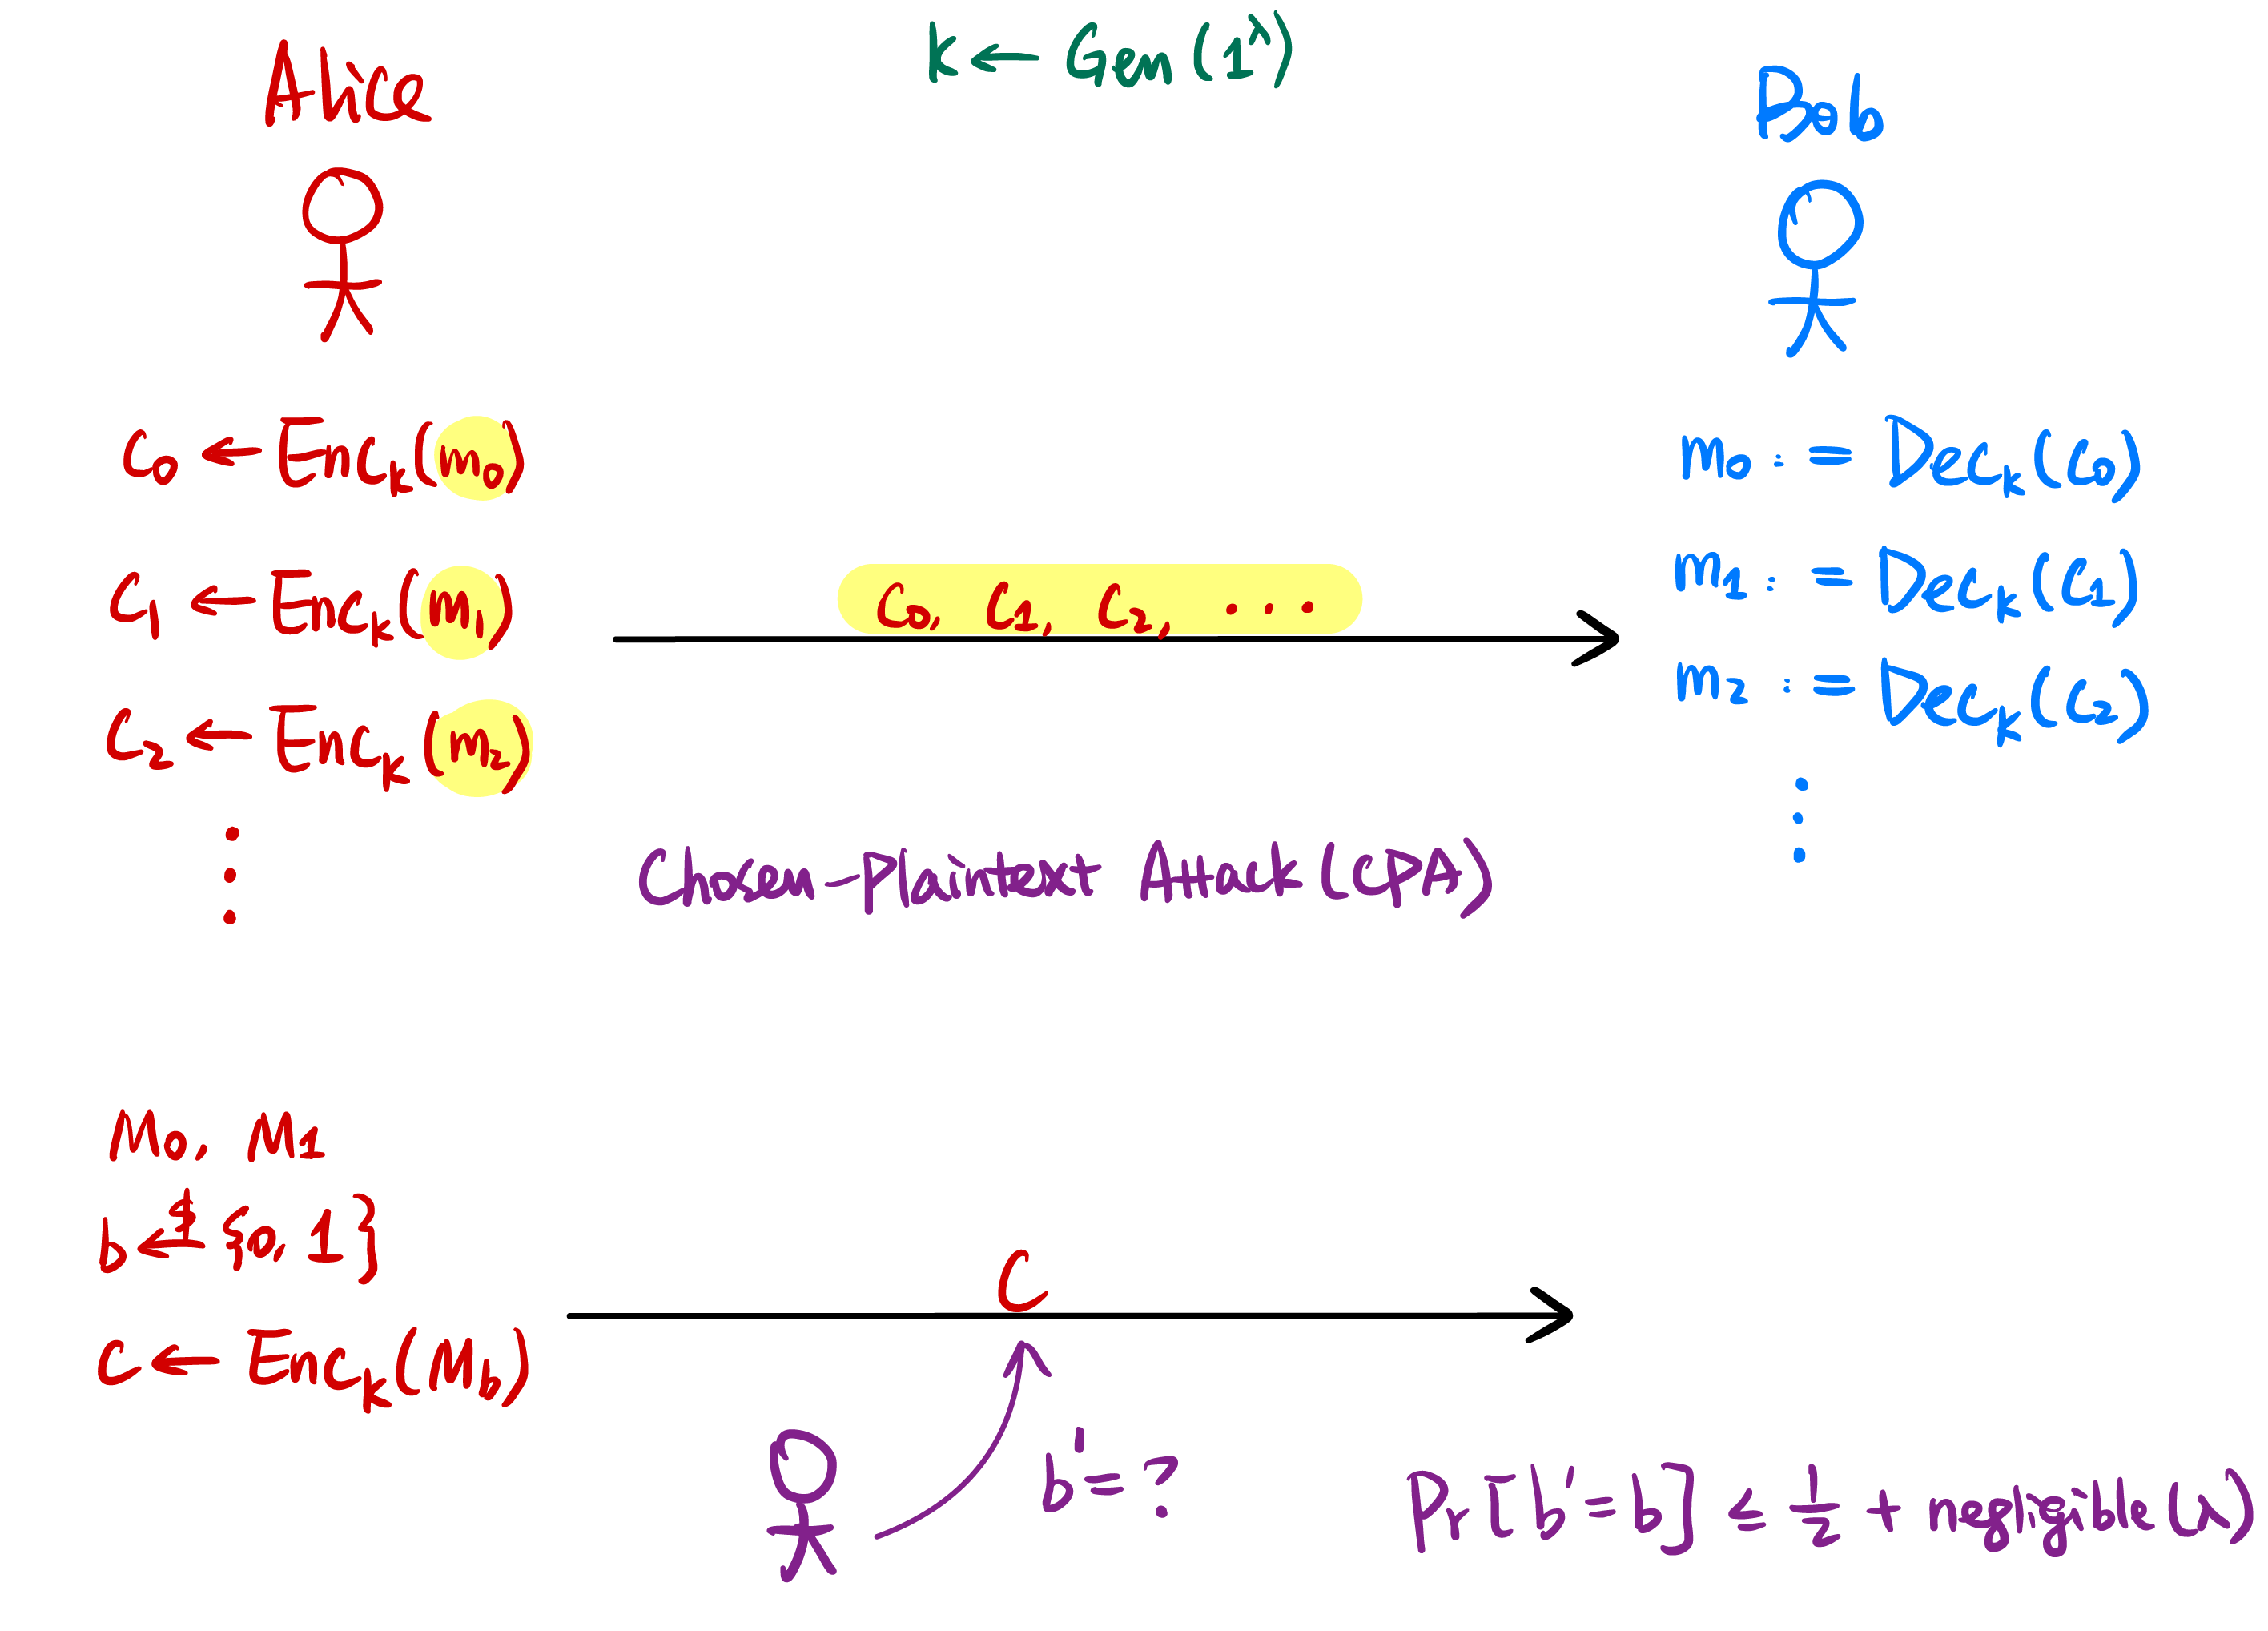
\includegraphics[width=0.8\textwidth]{images/2023-01-31/computational-security.png}
\end{center}

For a key generated $k\leftarrow \Gen(1^\lambda)$.

Theoretically, for $\lambda$ a security parameter and an adversary running in time $\mathsf{poly}(\lambda)$, the adversary should have distinguishing advantage $\negligible(\lambda)$ where
\[\negligible(\lambda) \ll \frac{1}{\lambda^c}\qquad \forall\text{ constant }c.\]

In practice, we set $\lambda = 128$. This means that the best algorithm to break the scheme (e.g. find the secret key) takes time $\sim 2^\lambda$. Currently, this is longer than the age of the universe.

\begin{example}
    \textbf{If the best algorithm is a brute-force search for $k$, what should our key length be?}

    It can just be a $\lambda$ bit string.
\end{example}
\begin{example*}
    \textbf{What if the best algorithm is no longer a brute-force search, but instead for a key length $l$ takes $\sim \sqrt{2^l}$?}

    Our key length should be $2\lambda$. Doing the math, we want $\sqrt{2^l} \equiv 2^\lambda$, solving for $l$ gives $2\lambda$.
\end{example*}

Going back to the original problem of secret-key encryption, how can we use our newfound cryptographic constructions to improve this?

From a pseudorandom function/permutation (PRF/PRP), we can reuse our secret key by passing it through the pseudorandom function.

The current practical construction for PRD/PRP is called the block cipher, and the standardized implementation is AES\footnote{Determined via a competition for such an algorithm in the early 2000s. }

It is a computational assumption\footnote{Based on heuristic, not involving any number theory!} that the AES construction is secure, and the best attack is currently a brute-force search (in both classical and quantum computing realms).

\subsubsection{Public-Key Encryption Schemes}
Using computational assumptions, we explore some public-key encryption schemes.

\begin{description}
    \item[RSA Encryption.] This is based on factoring/RSA assumption, that factoring large numbers is hard.
    \item[ElGamal Encryption.] This is based on the discrete logarithm/Diffie-Hellman Assumption, that finding discrete logs in $\ZZ_p$ is hard.
    \item[Lattice-Based Encryption.] The previous two schemes are not quantum secure. Quantum computation will break these schemes. Lattice-based encryption schemes are post-quantum secure. They are associated with the difficulty of finding `short' vectors in lattices\footnote{Covered later in class, we focus on the first two now.}.
\end{description}

Another thing worth mentioning is that
\begin{theorem}
    \emph{(Very informally,)} It is impossible to construct PKE from SKE in a black-box way. This is called ``black-box separation''.
\end{theorem}

We first need to define a bit of number-theory background.
\begin{definition}
    We denote $a\mid b$ as $a$ \ul{divides} $b$, that is, there is integer $c$ such that $b = a\cdot c$.
\end{definition}
\begin{definition}
    The $\gcd(a, b)$ is the greatest common divisor of $a, b$. If $\gcd(a, b) = 1$, then $a, b$ are coprime.
\end{definition}
\begin{ques*}
    How do we compute $\gcd$? What is its time complexity?
\end{ques*}
\begin{example*}
    We use the Euclidean Algorithm. Take $\gcd(12, 17)$,
    \begin{align*}
        17\mod{12} & = 5 \\
        12 \mod{5} & = 2 \\
        5\mod{2}   & = 1 \\
        2\mod{1}   & = 0
    \end{align*}
    or take $\gcd(12, 18)$
    \begin{align*}
        18\mod{12} & = 6 \\
        12\mod{6}  & = 0
    \end{align*}
\end{example*}
If we have two bitstrings of length $n$ bits, what is the running time of the Euclidan Algorithm?

\begin{center}
    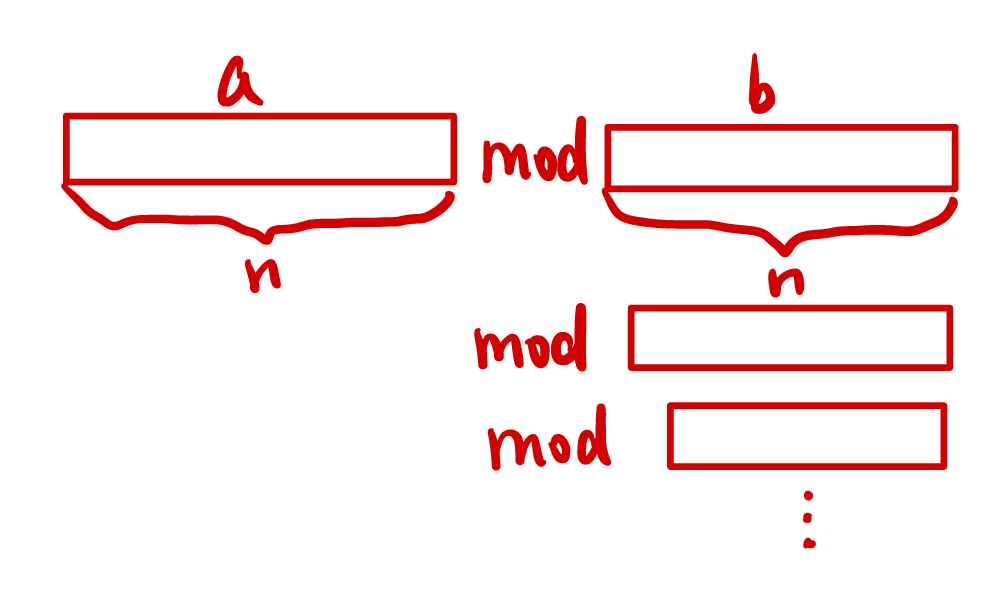
\includegraphics[width=0.3\textwidth]{images/2023-01-31/euclidean-algo.png}
\end{center}

Very informally, we see that every step, the length of $a, b$ decrease by approximately $1$ bit. Then, finding $\gcd$ is roughly order $O(n)$.

\begin{definition}[Mod]
    $a\mod{N}$ is the remainder of $a$ when divided by $N$.

    $a\equiv b\pmod{N}$ means when $a$ and $b$ are \ul{congruent modulo} $N$. That is, $a\mod N = b\mod N$.
\end{definition}

\begin{ques*}
    How might we compute $a^b\mod N$? What is the time complexity? Let $a, b, N$ be $n$-bit strings.
\end{ques*}

Na\"ively, we can repeatedly multiply. But this takes $b$ steps ($2^n$).

We can `repeatedly square'. For example, we can get to $a^8$ faster by getting $a^2$, squaring to get $a^4$, and again to get $a^8$. We can take the bitstring of $b$ and determine how to compute this.

\begin{example*}
    If $b = 100101_2$, we take $a\cdot a^4\cdot a^{32}\mod N$ which can be calculated recursively (an example is given in the first assignment).
\end{example*}

The time complexity of this is order $O(n)$ for $n$-bit $a, b, N$\footnote{Not exactly order $n$, we should add the complexity of multiplication. However, this should be bounded by $N$ since we can log at every step.}.

\begin{theorem}[Bezout's Theorem, \emph{roughly}]
    If $\gcd(a,N) = 1$, then $\exists b$ such that
    \[a\cdot b \equiv 1\pmod{N}.\]
    This is to say, $a$ is \ul{invertible modulo} $N$. $b$ is its inverse, denoted as $a^{-1}$.
\end{theorem}
\begin{ques*}
    How do we compute $b$?
\end{ques*}
We can use the Extended Euclidean Algorithm!
\begin{example*}
    We write linear equations of $a$ and $N$ that sum to $1$, using our previous Euclidean Algorithm. Take the previous example $\gcd(12, 17)$,
    \begin{align*}
        17\mod{12} & = 5 \\
        12 \mod{5} & = 2 \\
        5\mod{2}   & = 1 \\
        2\mod{1}   & = 0
    \end{align*}
    We write this as
    \begin{align*}
        5 & = 17 - 12\cdot 1                         \\
        2 & = 12 - 5\cdot 2 = 12\cdot x + 17\cdot y  \\
        1 & = 5 - 2\cdot 2 = 12\cdot x' + 17\cdot y'
    \end{align*}
    where we substitute the linear combination of $5$ into $5$ on line $2$, substitute linear combination of $2$ into $2$ on line $1$, each producing another linear combination of $12, 17$.

    If $\gcd(a, N) = 1$, we use the Extended Euclidean Algorithm to write $1 = a\cdot x + N\cdot y$, then $1\equiv a\cdot x\pmod{N}$.
\end{example*}

\begin{definition}[Group of Units mod $N$]
    We have set
    \[\ZZ_N^\times:= \left\{ a\mid a\in [1, N-1], \gcd(a, N) = 1 \right\}\]
    which is the group of units modulo $N$ (they are units since they all have an inverse by above).
\end{definition}
\begin{definition}[Euler's Phi Function]
    Euler's phi (or totient) function, $\phi(N)$, counts the number of elements in this set. That is, $\phi(N) =  |\ZZ_N^\times|$.
\end{definition}
\begin{theorem}[Euler's Theorem]
    For all $a, N$ where $\gcd(a, N) = 1$, we have that \[a^{\phi(N)} \equiv 1\pmod{N}.\]
\end{theorem}

With this, we can start talking about RSA.

\subsubsection{RSA}
We first define the RSA assumption.
\begin{definition}[Factoring Assumption]
    Given two $n$-bit primes $p, q$, we compute $N = p\cdot q$. Given $N$, it's computationally hard to find $p$ and $q$ (classically).
\end{definition}
\begin{definition}[RSA Assumption]
    Given two $n$-bit primes, we again compute $N = p\cdot q$, where $\phi(N) = (p-1)(q-1)$. We choose an $e$ such that $\gcd(e, \phi(N)) = 1$ and compute $d \equiv e^{-1}\pmod{\phi(N)}$.

    Given $N$ and a random $y\sampledfrom \ZZ_{N}^\times$, it's computationally hard to find $x$ such that $x^e\equiv y\pmod{N}$.

    \begin{center}
        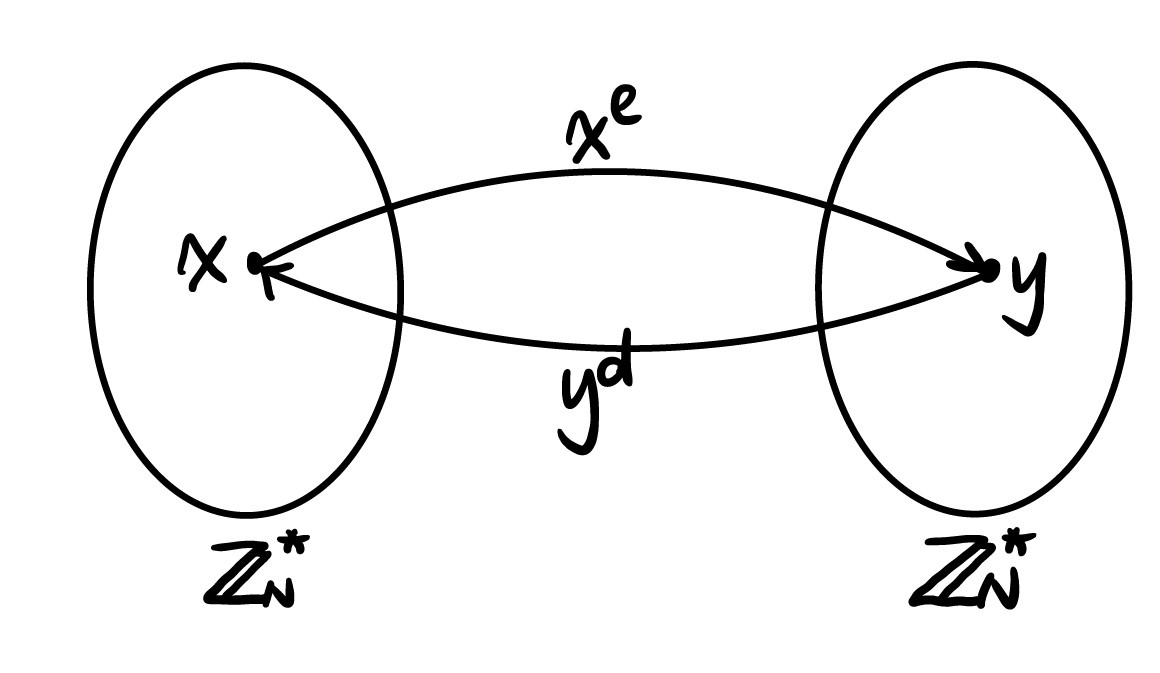
\includegraphics[width=0.4\textwidth]{images/2023-01-31/rsa.png}
    \end{center}

    However, given $p, q$, it's easy to find $d$. We know $\phi(N) = (p-1)(q-1)$, so we can compute $d$ from $e$ by running the Extended Euclidean Algorithm. Then, taking $(x^e)^d\equiv x^{ed}\equiv x$ which allows us to extract $x$ again.
\end{definition}

Encrypting is exactly raising by power $d$, and decrypting is raising again by power $e$.

Remaining questions:
\begin{itemize}
    \item How can we generate primes $p, q$?
    \item How can we pick $e$ such that $\gcd(e, \phi(N)) = 1$?
    \item What security issues can you see?
\end{itemize}

We'll continue next class.